%
%===============>>  ГРУППА 9-2 МОДУЛЬ 9 <<=============
%
\setmodule{9}

%BEGIN_FOLD % ====>>_____ Занятие 1 _____<<====
\begin{class}[number=1]
	\begin{listofex}
		\item Найдите значение выражения: \(\dfrac{ 9,4 }{ 4,1+5,3 }\).
		\item На координатной прямой отмечены числа \( a \) и \( b \). Какое из следующих утверждений неверно?
		\begin{center}
			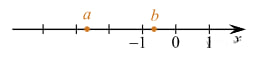
\includegraphics[align=t, width=0.5\linewidth]{\picpath/G93M8L6-6}
		\end{center}
		\begin{tasks}(2)
			\task \( a+b<0 \)
			\task \( -2<b-1<-1 \)
			\task \( a^2b<0 \)
			\task \( -a<0 \)
		\end{tasks}
		\item Найдите значение выражения \( \dfrac{a^{17}\cdot(b^5)^3}{(a\cdot b)^{15}} \) при \( a=7 \) и \( b=\sqrt{7} \).
		\item Решите уравнения: \(\dfrac{ 3 }{ x-19 }=\dfrac{ 19 }{ x-3 }\). \\
		Если корней несколько, запишите их в ответ без пробелов в порядке возрастания.
		\item В фирме такси в данный момент свободно \(15\) машин: \(3\) чёрных, \(6\) жёлтых и \(6\) зелёных. По вызову выехала одна из машин, случайно оказавшаяся ближе всего к заказчику. Найдите вероятность того, что к нему приедет жёлтое такси.
		\item На одном из рисунков изображен график функции \(y=x^2-2x+3\). Укажите номер этого рисунка.
		\begin{center}
			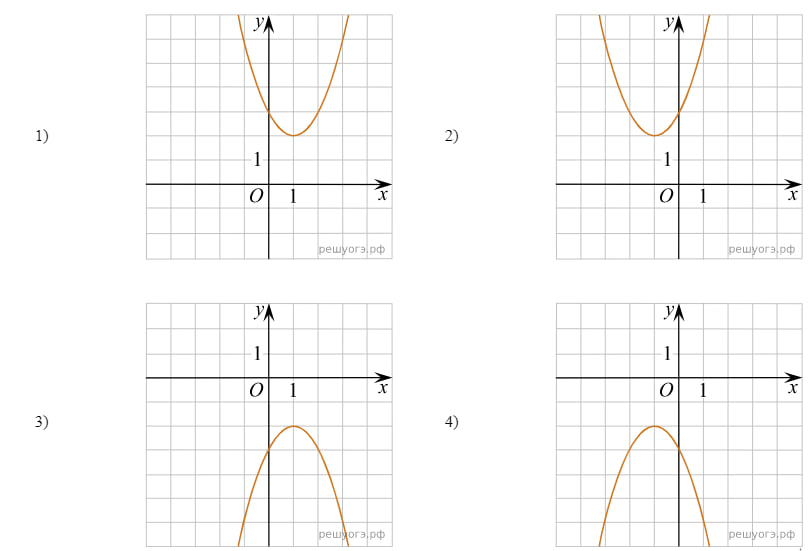
\includegraphics[align=t, width=0.9\linewidth]{\picpath/G91M9L1}
		\end{center}
		\item Объём пирамиды вычисляют по формуле \(V=\dfrac{ 1 }{ 3 }Sh\),  где \(S\) --- площадь основания пирамиды, \(h\) --- её высота. Объём пирамиды равен \(40\), площадь основания \(15\). Чему равна высота пирамиды?
		\item Решите неравенство: \(-x^2-2x\le0\).
		\item В амфитеатре \(14\) рядов. В первом ряду \(20\) мест, а в каждом следующем на \(3\) места больше, чем в предыдущем. Сколько мест в десятом ряду амфитеатра?
		\item В равностороннем треугольнике \(ABC\) биссектрисы \(CN\) и \(AM\) пересекаются в точке \(P\). Найдите \(\angle MPN\).
		\item К окружности с центром в точке \(O\) проведены касательная \(AB\) и секущая \(AO\). Найдите радиус окружности, если \(AB=12\) см, \(AO=13\) см.
		\item В треугольнике одна из сторон равна \(10\), другая равна \(10\sqrt{3}\), а угол между ними равен \(60\degree\). Найдите площадь треугольника.
		\item Основания трапеции равны \(18\) и \(12\), одна из боковых сторон равна \(4\sqrt{2}\), а угол между ней и одним из оснований равен \(135\degree\). Найдите площадь трапеции.
		\item Укажите номера верных утверждений.
		\begin{tasks}
			\task Если три угла одного треугольника равны трем углам другого треугольника, то такие треугольники подобны. 
			\task Сумма смежных углов равна \(180\degree\).
			\task Любая медиана равнобедренного треугольника является его биссектрисой.
		\end{tasks}
		\item Решите уравнение: \(x^2-2x+\sqrt{3-x}=\sqrt{3-x}+8\)
		\item Из пункта \(A\) в пункт \(B\), расстояние между которыми \(13\) км, вышел пешеход. Одновременно с ним из \(B\) в \(A\) выехал велосипедист. Велосипедист ехал со скоростью, на \(11\) км/ч большей скорости пешехода, и сделал в пути получасовую остановку. Найдите скорость пешехода, если известно, что они встретились в \(8\) км от пункта \(B\).
		\item Постройте график функции \(y=\dfrac{ (x+1)(x^2+7x+12) }{ x+3 }\) и определите, при каких значениях \(m\) прямая \(y=m\) имеет с графиком ровно одну общую точку.
		\item Периметр прямоугольника равен \(30\), а диагональ равна \(14\). Найдите площадь этого прямоугольника.
		\item Докажите, что медиана треугольника делит его на два треугольника, площади которых равны между собой.
		\item Основание \( AC \) равнобедренного треугольника \( ABC \) равно \( 12 \). Окружность радиуса \( 8 \) с центром вне этого треугольника касается продолжений боковых сторон треугольника и касается основания \( AC \) в его середине. Найдите радиус окружности, вписанной в треугольник \( ABC \).
	\end{listofex}
\end{class}
%END_FOLD

%BEGIN_FOLD % ====>>_____ Занятие 2 _____<<====
\begin{class}[number=2]
	\begin{listofex}
		\item Занятие 2
	\end{listofex}
\end{class}
%END_FOLD

%BEGIN_FOLD % ====>>_ Домашняя работа 1 _<<====
\begin{homework}[number=1]
	\begin{listofex}
		\item Домашняя работа 1
	\end{listofex}
\end{homework}
%END_FOLD

%BEGIN_FOLD % ====>>_____ Занятие 3 _____<<====
\begin{class}[number=3]
	\begin{listofex}
		\item Занятие 3 
	\end{listofex}
\end{class}
%END_FOLD

%BEGIN_FOLD % ====>>_____ Занятие 4 _____<<====
\begin{class}[number=4]
	\begin{listofex}
		\item Занятие 4
	\end{listofex}
\end{class}
%END_FOLD

%BEGIN_FOLD % ====>>_ Домашняя работа 2 _<<====
\begin{homework}[number=2]
	\begin{listofex}
		\item Решите систему уравнений: \( \begin{cases} x-y=-5; \\ x^2-2xy-y^2=17 \end{cases} \)
		\item Игорь и Паша красят забор за \( 8 \) часов. Паша и Володя красят этот же забор за \( 9 \) часов, а Володя и Игорь --- за \( 24 \) часа. За сколько минут мальчики покрасят забор, работая втроём?
		\item Постройте график функции \( y=|x+1|-|x-1|-x \) и найдите все значения \( k \), при которых прямая \( y=kx \) имеет с графиком данной функции ровно одну общую точку.
		\item Расстояние от точки пересечения диагоналей ромба до одной из его сторон равно \( 14 \), а одна из диагоналей ромба равна \( 56 \). Найдите углы ромба.
		\item 
		\begin{minipage}[t]{\bodywidth}
			Два равносторонних треугольника имеют общую вершину. Докажите, что отмеченные на рисунке отрезки \( AB \) и \( CD \) равны.
		\end{minipage}
		\gapwidth
		\begin{minipage}[t]{\picwidth}
			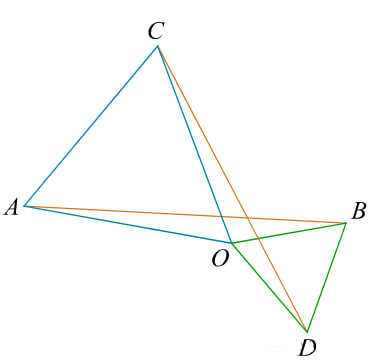
\includegraphics[align=t, width=\linewidth]{\picpath/G91M9H2}
		\end{minipage}
	\end{listofex}
\end{homework}
%END_FOLD

%BEGIN_FOLD % ====>>_____ Занятие 5 _____<<====
\begin{class}[number=5]
	\begin{listofex}
		\item Найдите значение выражения: \((4,9\cdot10^{-3})(4\cdot10^{-2})\).
		\item На координатной прямой отмечены числа \( a \) и \( b \). Какое из следующих утверждений неверно?
		\begin{center}
			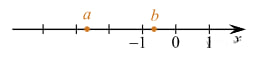
\includegraphics[align=t, width=0.5\linewidth]{\picpath/G93M8L6-6}
		\end{center}
		\begin{tasks}(2)
			\task \( a+b<0 \)
			\task \( -2<b-1<-1 \)
			\task \( a^2b<0 \)
			\task \( -a<0 \)8
		\end{tasks}
		\item Найдите значение выражения \( \dfrac{a^2-25b^2}{5ab}:\left( \dfrac{1}{5b}-\dfrac{1}{a} \right) \) при \( a=\mfrac{8}{1}{16} \), \( b=\mfrac{6}{3}{16} \).
		\item Решите уравнениe: \((x-11)(-x+9)=0\).
		\item Определите вероятность того, что при бросании игрального кубика (правильной кости) выпадет более \( 3 \) очков.
		\item Установите соответствие между графиками функций и формулами, которые их задают.
		\begin{center}
			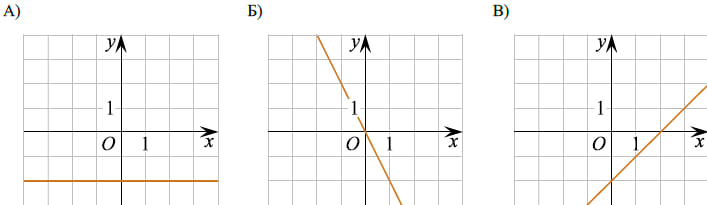
\includegraphics[align=t, width=0.7\linewidth]{\picpath/G91M9L5}
		\end{center}
		\begin{tasks}(3)
			\task \( y=-2 \)
			\task \( y=x-2 \)
			\task \( y=-2x \)
		\end{tasks}
		\item Закон всемирного тяготения можно записать в виде \( F=y\dfrac{m_1m_2}{r^2} \) где \( F \) --- сила притяжения между телами (в ньютонах), \( m_1 \) и \( m_2 \) --- массы тел (в килограммах), \( r \) --- расстояние между центрами масс (в метрах), а \( y \) --- гравитационная постоянная, равная \( 6,67\cdot10^{−11} \) H\( \cdot \)м\( ^2 \)/кг\( ^2 \). Пользуясь формулой, найдите массу тела (в килограммах), если \( F=1000,5 \) Н, \( m_2=6\cdot10^9 \) кг, а \( r=4 \) м.
		\item Решение какого из данных неравенств изображено на рисунке?
		\begin{center}
			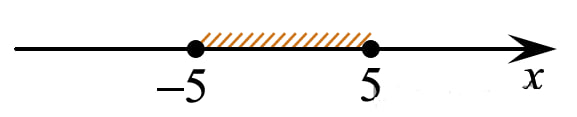
\includegraphics[align=t, width=0.5\linewidth]{\picpath/G91M9L5-1}
		\end{center}
		\begin{tasks}(4)
			\task \( x^2-25\le0 \)
			\task \( x^2+25\le0 \)
			\task\( x^2-25\ge0 \)
			\task \( x^2+25\ge0 \)
		\end{tasks}
		\item Мать дарит каждой из пяти своих дочерей в день рождения, начиная с пяти лет, столько книг, сколько дочери лет. Возрасты пяти дочерей составляют арифметическую прогрессию, разность которой равна \( 2 \). Сколько лет было старшей дочери, когда у них составилась библиотека общей численностью в \( 495 \) книг?
		\item 
		\begin{minipage}[t]{\bodywidth}
			Радиус окружности с центром в точке \( O \) равен \( 50 \), длина хорды	\( AB \) равна \( 80 \) (см. рис.). Найдите расстояние от хорды \( AB \) до параллельной ей касательной \( k \).
		\end{minipage}
		\gapwidth
		\begin{minipage}[t]{\picwidth}
			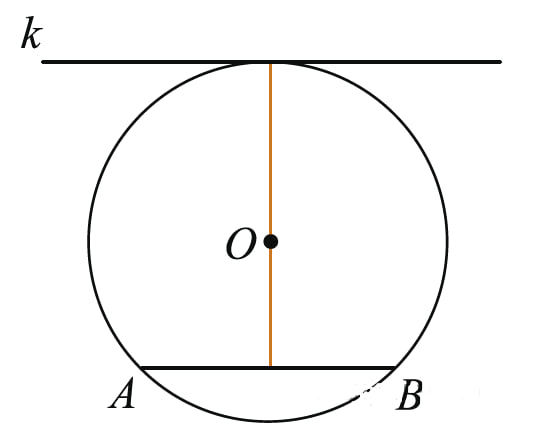
\includegraphics[align=t, width=\linewidth]{\picpath/G91M9L5-2}
		\end{minipage}
		\item Окружность с центром в точке \( O \) описана около равнобедренного треугольника \( ABC \), в котором \( AB=BC \) и \( \angle ABC=79\degree \). Найдите величину угла \( BOC	 \). Ответ дайте в градусах.
		\item Сторона треугольника равна \( 14 \), а высота, проведённая к этой стороне, равна \( 31 \). Найдите площадь этого треугольника.
		\item
		\begin{minipage}[t]{\bodywidth}
			На клетчатой бумаге с размером клетки \( 1X1 \) изображён параллелограмм. Найдите его площадь.
		\end{minipage}
		\gapwidth
		\begin{minipage}[t]{\picwidth}
			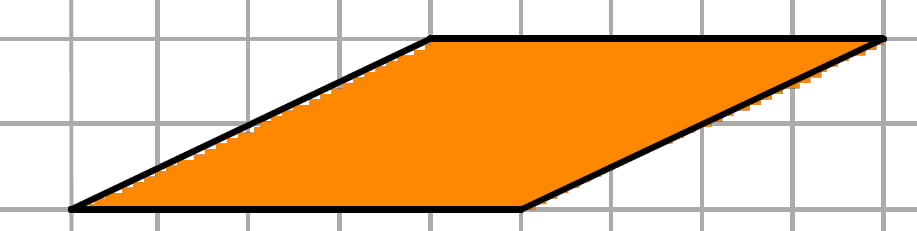
\includegraphics[align=t, width=\linewidth]{\picpath/G91M9L5-3}
		\end{minipage}
		\item Какое из следующих утверждений верно?
		\begin{tasks}
			\task Если диагонали параллелограмма равны, то этот параллелограмм является ромбом.
			\task Тангенс любого острого угла меньше единицы.
			\task Сумма углов равнобедренного треугольника равна 180 градусам.
		\end{tasks}
		\item Сократите дробь: \( \dfrac{ab-3a-2b+6}{a^2-4} \)
		\item Баржа прошла по течению реки \( 72 \) км и, повернув обратно, прошла ещё \( 54 \) км, затратив на	весь путь \( 9 \) часов. Найдите собственную скорость баржи, если скорость течения реки равна \( 5 \) км/ч.
		\item Постройте график функции \( y=4|x+6|-x^2-11x-30 \) и определите, при каких значениях \( m \)	прямая \( y=m \) имеет с графиком ровно три общие точки.
		\item Высота \( AH \) ромба \( ABCD \) делит сторону \( CD \) на отрезки \( DH=24 \) и \( CH=6 \). Найдите высоту ромба.
		\item Известно, что около четырёхугольника \( ABCD \) можно описать окружность и что продолжения сторон \( AD \) и \( BC \) четырёхугольника пересекаются в точке \( K \). Докажите, что треугольники \( KAB \) и \( KCD \) подобны.
	\end{listofex}
\end{class}
%END_FOLD

%BEGIN_FOLD % ====>>_____ Занятие 6 _____<<====
\begin{class}[number=6]
	\begin{listofex}
		\item Занятие 6
	\end{listofex}
\end{class}
%END_FOLD

%BEGIN_FOLD % ====>>_ Домашняя работа 3 _<<====
\begin{homework}[number=3]
	\begin{listofex}
		\item Решите систему неравенства:
		\[\begin{cases} \dfrac{10-2x}{3+(5-2x)^2}\ge0,\\2-7x\le14-3x \end{cases}\]
		\item Первые \( 300 \) км автомобиль ехал со скоростью \( 60 \) км/ч, следующие \( 300 \) км --- со скоростью \( 100 \) км/ч, а последние \( 300 \) км --- со скоростью \( 75 \) км/ч. Найдите среднюю скорость автомобиля на протяжении всего пути.
		\item Постройте график функции \( y=\dfrac{|x|-4}{x^2-4|x|} \) и определите, при каких значениях \( k \) прямая \( y=kx \) не будет иметь с построенным графиком ни одной общей точки.
		\item Диагонали \( AC \) и \( BD \) трапеции \( ABCD \) пересекаются в точке \( O \). Площади треугольников \( AOD \) и \( BOC \) равны соответственно \( 16 \) см\( ^2 \)  и 9 см\( ^2 \). Найдите площадь трапеции.
		\item В равнобедренном треугольнике \( ABC \) (\( AB=BC \)) точки \( M \), \( N \), \( K \) --- середины сторон \( AB \), \( BC \), \( CA \) соответственно. Докажите, что треугольник \( MNK \) --- равнобедренный.
	\end{listofex}
\end{homework}
%END_FOLD

%BEGIN_FOLD % ====>>_____ Занятие 7 _____<<====
\begin{class}[number=7]
	\title{Подготовка к проверочной}
	\begin{listofex}
		\item Занятие 7
	\end{listofex}
\end{class}
%END_FOLD

%BEGIN_FOLD % ====>>_ Проверочная работа _<<====
\begin{exam}
	\begin{listofex}
		\item Проверочная
	\end{listofex}
\end{exam}
%END_FOLD

%BEGIN_FOLD % ====>>_ Домашняя работа 4 _<<====
\begin{homework}[number=4]
	\begin{listofex}
		\item В амфитеатре \( 10 \) рядов. В первом ряду \( 25 \) мест, а в каждом следующем на \( 3 \) места больше, чем в предыдущем. Сколько мест в восьмом ряду амфитеатра?
		\item 
		\begin{minipage}[t]{\bodywidth}
			В кафе есть только квадратные столики, за каждый из которых могут сесть \( 4 \) человека. Если сдвинуть два квадратных столика, то получится стол, за который могут сесть \( 6 \) человек. На рисунке изображён случай, когда сдвинули \( 3 \) квадратных столика вдоль одной линии. В этом случае получился стол, за который могут сесть \( 8 \) человек. Сколько человек может сесть за стол, который получится, если сдвинуть \( 16 \) квадратных столиков вдоль одной линии?
		\end{minipage}
		\hspace{0.02\linewidth}
		\begin{minipage}[t]{\picwidth}
			% TODO: \usepackage{graphicx} required
			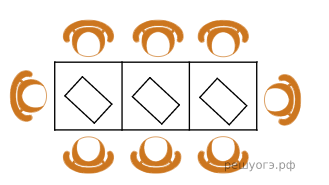
\includegraphics[align=t, width=\linewidth]{../../../../../exercises/lists/pics/leontevaM9L4-4}
		\end{minipage}
		\item Диагональ \( AC \) параллелограмма \( ABCD \) образует с его сторонами углы, равные \( 25\degree \) и \( 30\degree \). Найдите больший угол параллелограмма.
		\item Точка \( O \) --- центр окружности, на которой лежат точки \( P \), \( Q \) и \( R \) таким образом, что \( OPQR \) --- ромб. Найдите угол \( ORQ \). Ответ дайте в градусах.
		\item Основания трапеции равны \( 18 \) и \( 12 \), одна из боковых сторон равна \( 6 \), а тангенс угла между ней и одним из оснований равен \( \dfrac{\sqrt{2}}{4} \).  Найдите площадь трапеции.
		\item Найдите площадь квадрата, если его диагональ равна \( 3 \).
		\item Укажите номера верных утверждений.
		\begin{tasks}(1)
			\task Через точку, не лежащую на данной прямой, можно провести прямую, параллельную этой прямой.
			\task Треугольник со сторонами \( 1 \), \( 2 \), \( 4 \) существует.
			\task Если в ромбе один из углов равен \( 90\degree \), то такой ромб --- квадрат.
			\task Центр описанной около треугольника окружности всегда лежит внутри этого треугольника.
		\end{tasks}
		\item Решите уравнение: \( (x^2-16)^2+(x^2+x-12)^2=0 \)
		\item Расстояние между пристанями \( A \) и \( B \) равно \( 108 \) км. Из \( A \) в \( B \) по течению реки отправился плот, а через час вслед за ним отправилась моторная лодка, которая, прибыв в пункт \( B \), тотчас повернула обратно и возвратилась в \( A \). К этому времени плот прошёл \( 50 \) км. Найдите скорость лодки в неподвижной воде, если скорость течения реки равна \( 5 \) км/ч.
	\end{listofex}
\end{homework}
%END_FOLD